\section{Introduction \& Background}
In 2018 there was approximately 261$\si{\tera\watt\hour}$ of power generation in the Australian electricity sector. Renewables contributed to 19\% of the total generation, increasing from 15\% in 2017 \cite{Diser2020}. This is a pattern which has followed on from 2016. Indeed, a trend of greater renewable energy penetration in the electricity generation market has emerged starting in approximately 2008, as shown in Figure 1.
\begin{figure}[ht]
	\centering
	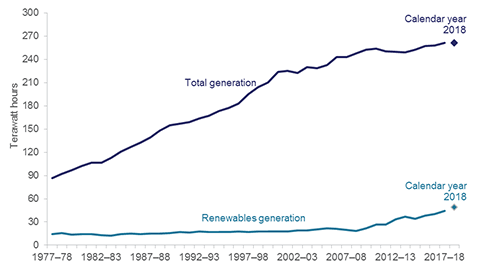
\includegraphics[height=7cm]{australian_generation_profile}
	\caption{text}
\end{figure}

One of the benefits of transitioning from thermal sources of generation to renewable sources is reduced greenhouse gas emissions (REFERENCE), however, this transition is not without its drawbacks. Increased reliance on renewable generation sources poses some challenges regarding power system stability. A recent example is the system failure resulting from an event cascade, triggered by cloud cover shadowing a solar array in Alice Springs. The system failure resulted in a blackout occurring in Alice Springs for approximately 8 hours (REFERENCE). The Entura report highlighted that poor control policies were one of the many factors contributing to the blackout. In this instance, a generator provisioned to ramp up in the event of cloud cover limiting solar array output was unable to be controlled (REFERENCE). Moreover, generators that were still under the control regime were issued operating set points above their rated capacity, which eventually resulted in thermal overload and subsequent tripping from the protection system.

One of the issues with currently employed control methods (using classical techniques) is that they can be brittle when faced with system changes, or scenarios which they were not designed for/ envisioned. A more robust controller would be one that can learn and adapt to a system, given some broad control objective. (NEED TO REPHRASE THIS ASPECT). This research proposes a Deep Reinforcement Learning agent for controlling the frequency of a power system with multiple generators, and multiple stochastic loads. Existing approaches currently employ classical engineering control methodologies.

\subsection{Power Systems and Frequency}
Interconnected power systems are comprised of power generating units and energy storage systems connected to transmission and distribution networks. Generated power is used to service load demand. A single line diagram of a power network can be seen in Figure 1. The left hand side of the diagram shows thermal generation units, such as coal and nuclear, in addition to renewable sources of generation, like wind and solar. The right hand side of the figure shows the distribution network and the consumers of generated energy: industry and households.
\begin{figure}[ht]
	\centering
	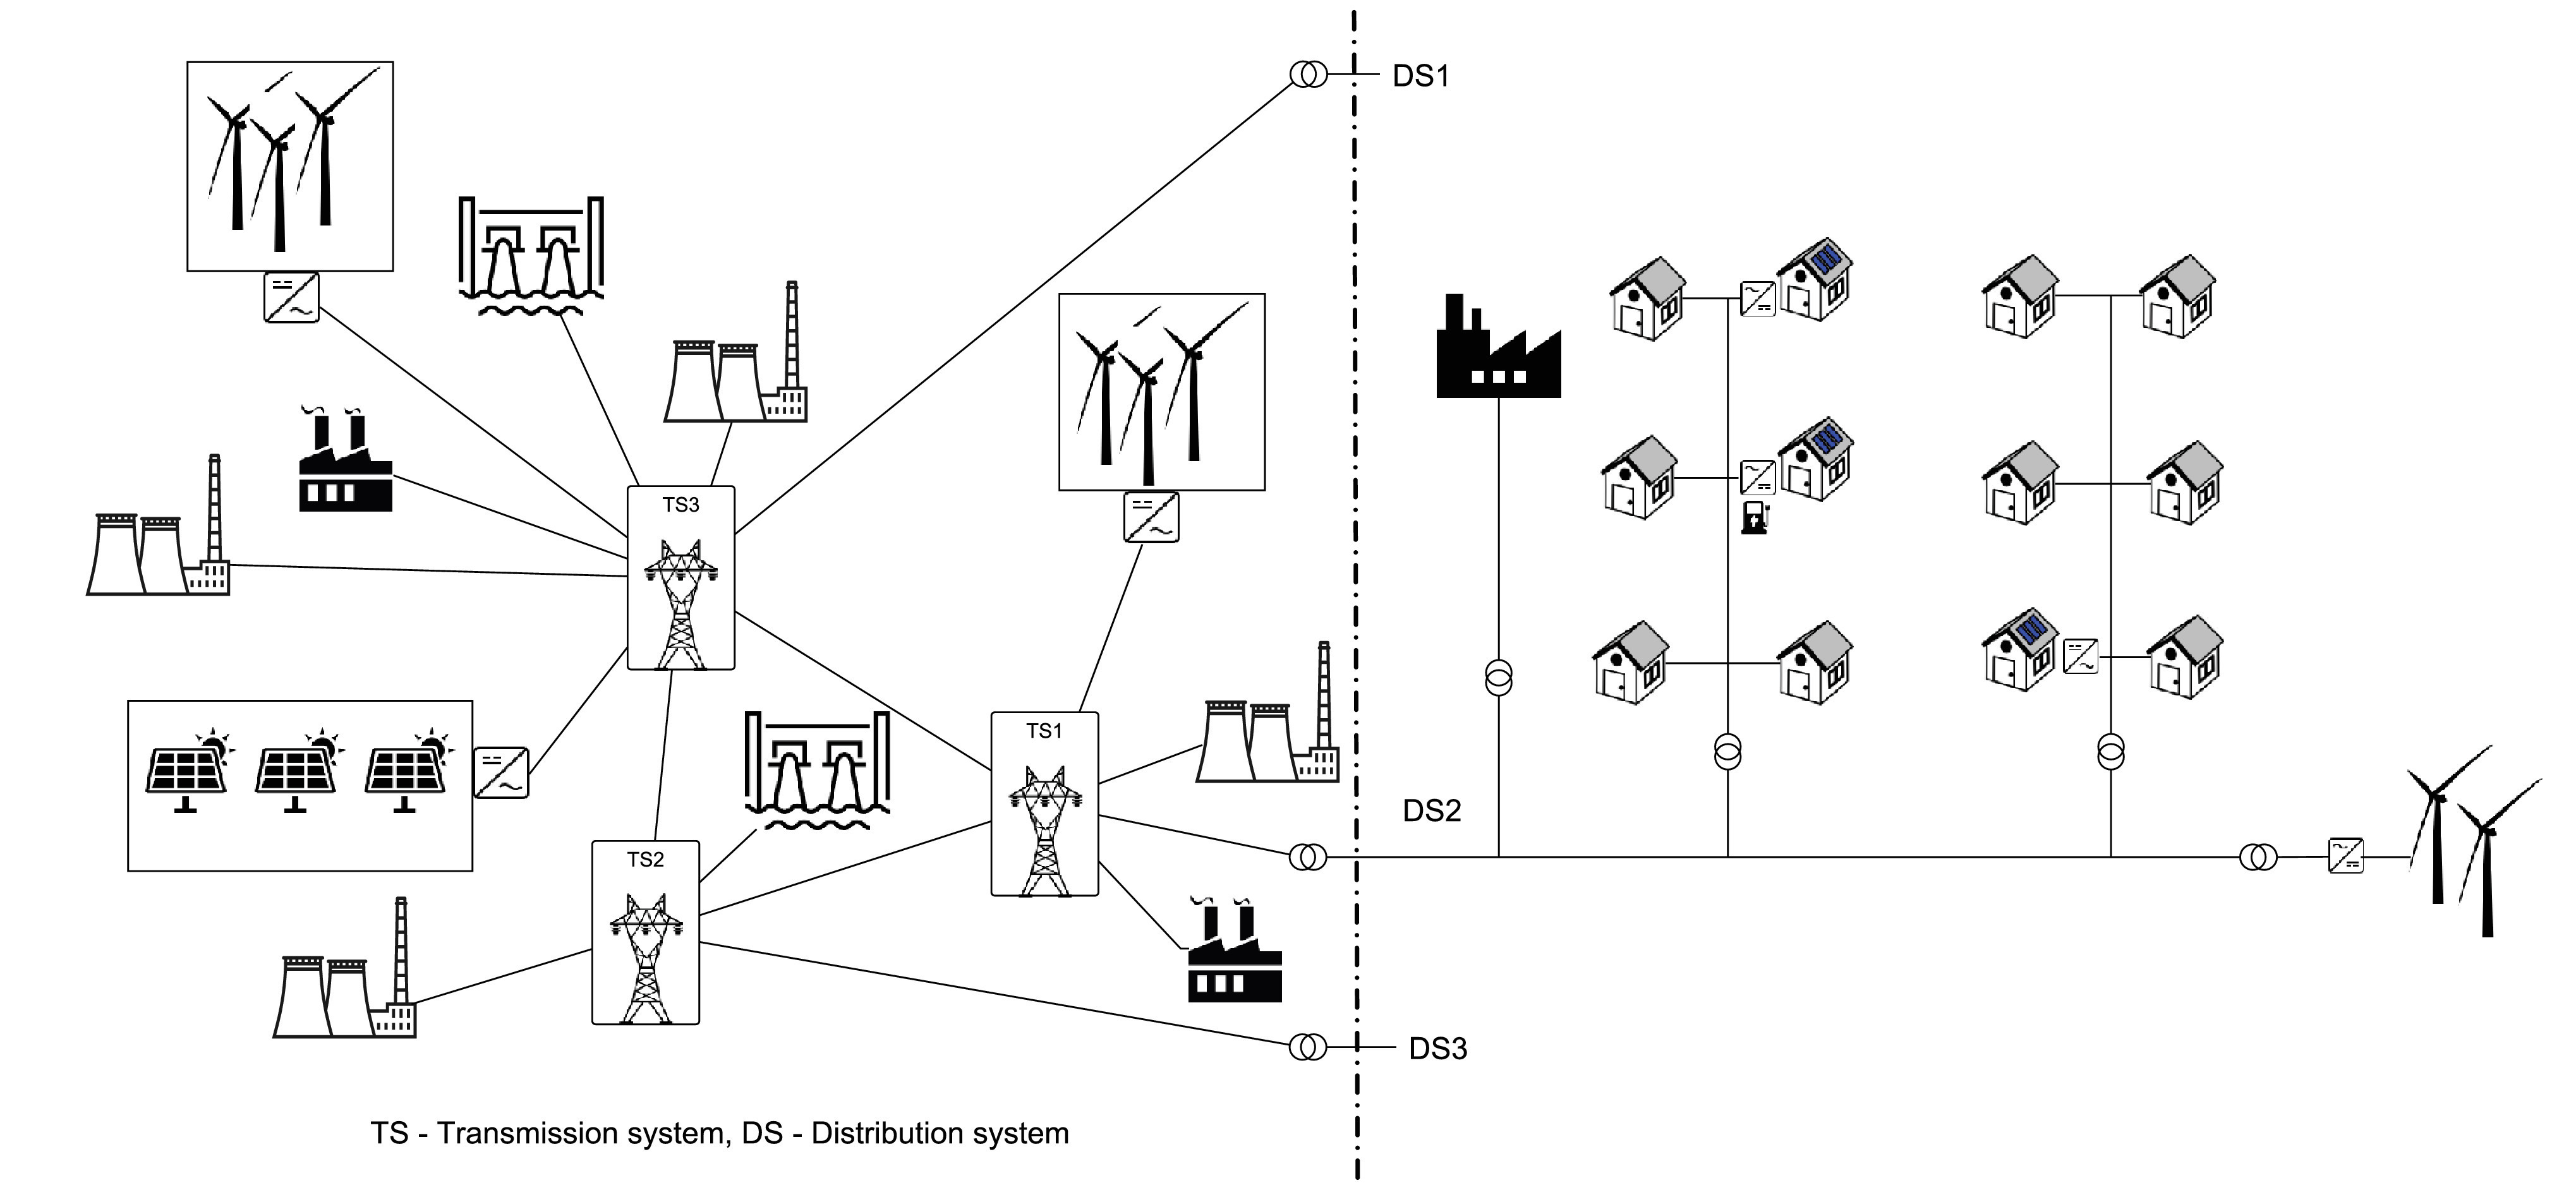
\includegraphics[scale=0.85]{power_system}
	\caption{A single line diagram of a typical power system taken from \cite{Glavic2019}. The image shows points of generation from thermal and renewable sources, and the subsequent supply of generated energy to meet load demand through the transmission and distribution network.}
\end{figure}

One of the key elements to successful operation of interconnected power systems is ensuring total load demand is matched with total generation, taking into account power losses involved with generation, transmission, and distribution \cite{Wood2013}. To understand why it is important to match generation with load demand it is useful to first consider the basic operation of a single thermal generator. 
\begin{figure}[h]
\centering
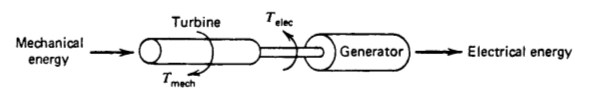
\includegraphics[height=1.4cm]{generation}
\caption{A thermal generation unit consists of a prime mover (turbine), and a synchronous machine. This image was taken from \cite{Wood2013}.}
\end{figure}

The essential elements of a thermal generator are a prime mover (turbine) and a synchronous machine, as depicted in Figure 2. The prime mover provides mechanical torque, $T_{mech}$, which drives the synchronous machine producing electrical energy. In response, the synchronous machine creates a torque which opposes $T_{mech}$, dependent on the size of the load demand from households and industry. This is referred to as electrical torque and is denoted as $T_{elec}$. If $\alpha$ represents angular acceleration of the generator rotating mass, and $I$ is its moment of inertia, then by Newton's second law:
\begin{equation}
\sum T_i = I \alpha 
\end{equation}

Equation (1) shows that when $T_{mech}$ equals $T_{elec}$ the system will be in a steady state with zero angular acceleration, and a constant rotation at some angular velocity $\omega$. Now, if $T_{mech} > T_{elec}$, then the angular velocity $\omega$ of the system will increase as the system speeds up, resulting in a frequency increase in the system. Conversely, if $T_{mech} < T_{elec}$ then the angular velocity $\omega$ will decrease as the system slows down, resulting in a frequency decrease. What makes this situation interesting is that at any point in time the total electrical load demand will fluctuate stochastically, meaning that an uncontrolled system will have a continually changing frequency. Australia's electricity network is designed to operate at a frequency of 50$\si{\hertz}$. In the majority of network scenarios AEMO has a desired operating range for frequency which lies between 49.85$\si{\hertz}$ and 50.15$\si{\hertz}$ \cite{AEMOfreqdev}. Similarly, the PWC Network Technical Code for the Northern Territory states that under normal operating conditions frequency should be maintained in the range 49.80$\si{\hertz}$ to 50.20$\si{\hertz}$ \cite{Pwc2013}. Operation outside of specified ranges can cause damage to electrical equipment such as transformers or motors, which are designed to operate at specific frequencies \cite{Sen2014}. Network designers engineer protection schemes so that sustained frequency excursions outside of the allowed range will cause equipment to trip from the network \cite{AEMOpowerfreqriskrev}. Protection schemes tripping equipment from the network is undesirable since this can leave households and industry without power, resulting in economic loss. Further, if disconnections are uncontrolled then this can lead to a further loss of system stability \cite{AEMOpowerfreqriskrev}.

\begin{figure}[ht]
	\centering
	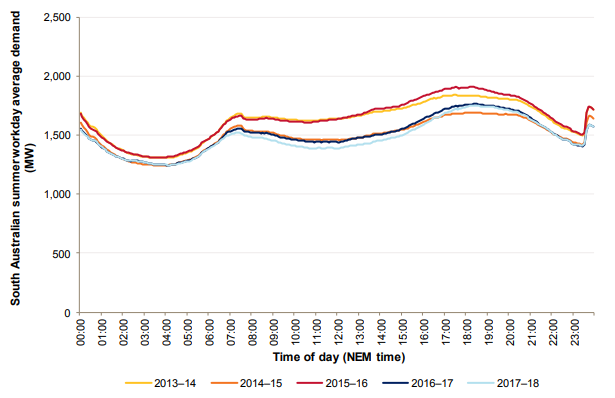
\includegraphics[height=7cm]{load_profile}
	\caption{Weekday energy demand profile in South Australia during summer \cite{Aemosaenergyrep}.}
\end{figure}

System controllers, such as the Australian Energy Market Operator (AEMO) and Power and Water Corporation (PWC), are therefore interested in being able to control the system to follow changes in load demand so that system frequency is maintained in the allowable range. Additionally, they are interested in control mechanisms to restore frequency excursions as a result of unexpected disturbances. System controllers can use historical data to forecast daily demand profiles with some reliability. A plot of average historical data, for the daily demand profile in South Australia during Summer, can be seen in Figure 3. This type of forecasting does not help when trying to predict the occurrence of random disturbances, however, it does provide a starting point for estimating required generation needed to meet demand. It is important to note that forecasting is not perfect. Inevitably mismatches in supply and demand will occur causing small imbalances between $T_{mech}$ and $T_{elec}$, resulting in a change to angular velocity $\omega$ and the network frequency \cite{Glover2012}. To perfectly match supply and demand, system controllers use generators referred to as regulating units \cite{Kothari2011}. A regulating unit is a generator that has capacity to increase or decrease mechanical torque $T_{mech}$ allowing the system controller to provide two functions: load following; and restoring the system to stable operating conditions in the event of a disturbance \cite{Grainger1994}. Using a regulating unit to load follow is referred to as the provision load following ancillary services \cite{AEMOancilliaryserv}. Load following control adjusts regulating units slightly to match supply perfectly with a demand load profile, like that shown in Figure 3. Using a regulator to restore the system after a disturbance is referred to as providing spinning reserves \cite{AEMOancilliaryserv}. When used in this fashion the regulating unit is not responsible for arresting frequency excursions, rather, it is used to restore the system back to the allowable frequency operating range after the frequency excursion has been arrested. An example of a frequency excursion, arrest, and subsequent restoration can be seen in Figure XXXX.

\begin{figure}[ht]
\centering
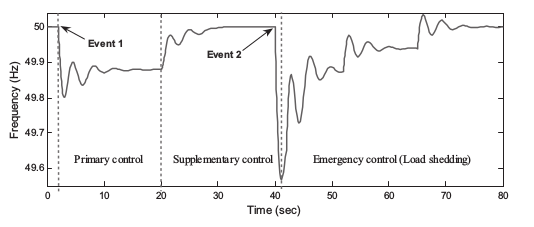
\includegraphics[height=8cm]{frequency_arrest}
\caption{A frequency disturbance occurs just before the 10 second mark, and regulating units ramp up their generation to first arrest the disturbance, and provide the subsequent correction, returning system frequency to 50$\si{\hertz}$.}
\end{figure}

AEMO and PWC do not require all generators on the network to act as regulating units since adequate frequency control can be achieved using a subset of the available generators.

\subsection{Frequency control for a single area system}
The power system model shown in Figure 1, on page 2, depicts total generation coming from many generation assets - this is complex to model. Researchers often find it useful to divide generation assets into sub-groups referred to as control areas \cite{Kothari2011}. A control area is defined as a subset of generators which are in close proximity to each other and constitute a coherent group that speed up and slow down together, maintaining their relative power angles \cite{Kothari2011}. The total network is therefore comprised of many interconnected control areas. An example of a series of interconnected control areas can be seen in Figure 5. Notice that for each area there is only a single load and a single generator. Typically, for each control area, researchers will aggregate many loads into a single load, and many generators into a single generator. This simplifies the model further \cite{Grainger1994}.
\begin{figure}[ht]
	\centering
	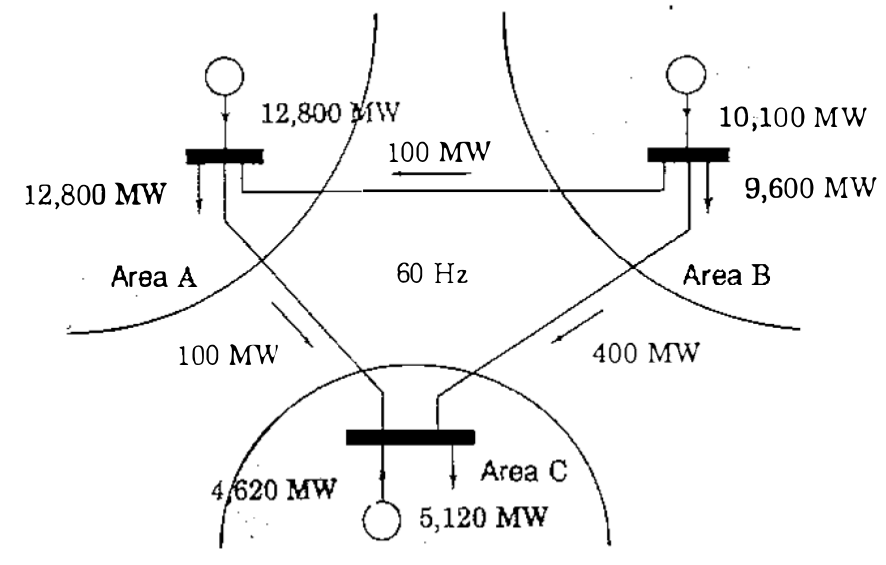
\includegraphics[height=8cm]{multiple_area_system}
	\caption{An example of three interconnected control areas in a 60$\si{\hertz}$ power system. The interconnections allow power to flow from one area to another, allowing generators to service loads from different areas. Each control area is consists of many generators and loads, but are modelled with a single generator and single load, respectively \cite{Grainger1994}.}
\end{figure}

The simplest power system to control is one that consists of a single control area, such as Area A in Figure 5. This power system has no interconnections to any other control area. It is comprised of consumer load demand, and a set of generators, some of which are acting as regulating units. As previously mentioned, for modelling simplicity, loads are aggregated to a single load, and generators are aggregated to a single generator. This classic, simple system is well understood and it is generally acknowledged that a governor feedback control regime can successfully perform frequency control of the system \cite{Wood2013, Grainger1994, Kothari2011}. Most introductory textbooks on power systems cover governor control of this system. Kothari (2011) provides a particularly well laid out approach to developing linear models for the turbine, generator load, and governor for the system - the full model can be seen in Figure 6 \cite{Kothari2011}. The leftmost block is a first-order linear model of the speed governor, the second block is a first-order model of the turbine, which the controller directly acts on. The final block is the generator load, which is also a first order system. The over all system model is a second order linear model, with a first order controller.

\begin{figure}[ht]
\centering
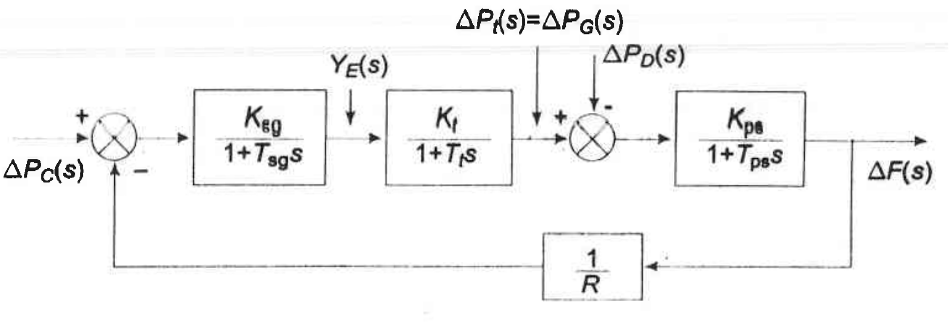
\includegraphics[height=5cm]{single_area_control}
\caption{A classical feed back control approach to a second order linear system. The second order system is comprised of a first order model for both the turbine, and generator load. The controller is modelled as a first order system \cite{Kothari2011}.}
\end{figure}


\subsection{Frequency control for two area system}
The system presented in Section 2.2 is useful to help understand the role of governors in controlling power system frequency, however, a single area model is too simple. In reality, power systems are comprised of many control areas connected through tie lines, which are typically transmission lines (REFERENCE). Often it is the case that there is some net power transfer over the tie lines, enforceable by contract. Distinct control areas are typically thought of as different participants in the generation market, or simply as different regions in which generation assets are based (REFERENCE). The simplest model which includes tie lines is the two area power system \cite{Kothari2011}.

\begin{figure}[ht]
	\centering
	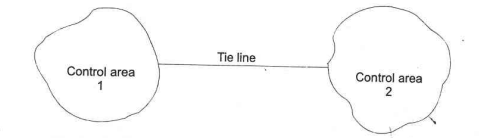
\includegraphics[height=3cm]{two_area_system}
	\caption{Two area power system is comprised of generators and load connected via a tie line. Power flows from one area to the other depending on economic contracts.}
\end{figure}

The control objective now is to maintain the inter-area power transfer, whilst regulating the frequency of each area. Simply relying on governor control in each area will not satisfy the control objective. Suppose control area 1 was supplying a 50MW load, and was contracted to supply control area 2 with 20MW. If control area 2 also has a 50MW load, then it is supplying only 30MW to satisfy the demand in this area. Now, consider a 30MW load increase in the demand for area 1. Relying on governor control will see generators from both area 1 and area 2 speed up in response to this step change. Ultimately, the increased power demands will be met, however, the power transfer over the tie line is likely to be less than the contracted 20MW value - this is problematic. Contract violations due to system instability and control issues do not allow for a stable market in which energy can be reliably traded. Fortunately, two area power systems are well understood. Linear models have been developed to simulate these systems, and classical control approaches have been successfully implemented to meet the new control objectives. In order to achieve this, a metric called Area Control Error (ACE) is used. This measures the distance from a target frequency as well as the deviation from tie-line contractual obligations. The implementation of this control system is shown in Figure XXXX.

\begin{figure}[ht]
	\centering
	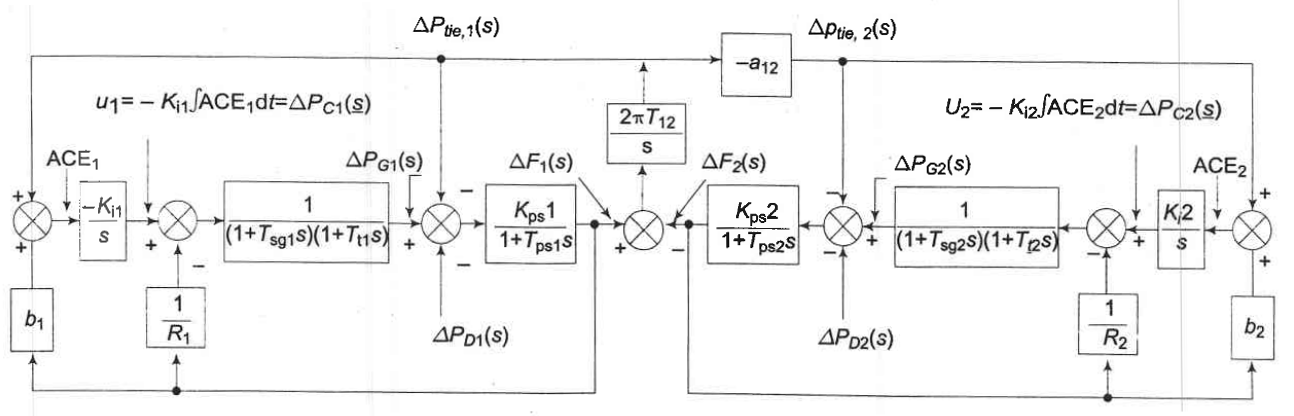
\includegraphics[height=4.8cm]{two_area_control_block}
	\caption{A classical feed back control approach to a two power area system \cite{Kothari2011}.}
\end{figure}


\subsection{Reinforcement learning}
Reinforcement Learning (RL) is a branch of machine learning that is concerned with how agents make sequential decisions to maximise some notion of a cumulative reward. It is a simple idea, but one which can be generalised to applications in many different fields, such as NOTE FIELDS HERE. Subsections 1.4.1 and 1.4.2 provide a brief overview of key architectural components of RL, and subsection 1.4.3 gives details on how these components are implemented to build an agent that can perform a control activity.

\subsubsection{Markov decision process}
Suppose that a robotic agent exists in some environment which is comprised of many discrete states, $s \in S$, such that $S$ denotes the state space. At any discrete point in time the agent can take an action $a \in A$, where $A$ denotes the action space. When the agent takes an action in a given state, the agent receives some reward, denoted with $r \in R$, where $R$ is the reward set. If an agent is in a given state, $s$, and takes and action, $a$, this will transition the agent to a new state, $s'$, and yield reward, $r$, with some given probability - these are referred to as state transition probabilities. Transition probabilities are denoted as follows:
\begin{equation}
P(S_{t+1}=s', R_{t+1}=r \ | \ S_t = s, A_t = a)
\end{equation}

The set of parameters, outlined above, make up a framework referred to as a Markov Decision Process (MDP) \cite{Sutton2018}.

\subsubsection{Return, episodes, and policy}
As the robotic agent takes actions at each discrete time step, it receives a reward. The cumulative sum of this reward is referred to as the return \cite{Sutton2018}. The return is denoted, for $N$ discrete time steps, as:
\begin{equation}
G_t = r_t + r_{1+1} + r_{t+2} + \ldots + r_{N-1}
\end{equation}

Often it is convenient to make future rewards less important than more immediate rewards. This is achieved by multiplying each reward in the sequence by a discount factor, $\gamma \in [0,1]$. Equation (XXXX) then becomes:
\begin{equation}
G_t = r_t + \gamma r_{1+1} + \gamma^2 r_{t+2} + \ldots + \gamma^{N-1} r_{N-1} = \sum_{k = 0}^{N-1} \gamma^k r_{t+k}
\end{equation}

Typically the duration of time that an agent will cumulate reward over is referred to as an episode. An episode is made up of a beginning, middle, and an end. Typically this consists of an RL agent beginning in some initial state, a period of time passes where the agent takes actions and undergoes state transitions, and then the episode concludes when the agent reaches a terminal state. At the episode conclusion, the agent receives it's cumulative reward.

Finally, in order for the robot to act within the environment, it needs to have a policy. A policy, $\pi$, is defined as a mapping from states to actions, that is, a rule which determines what action the robot will take for a given state. A deterministic policy, $\pi (s)$, maps a single action to a single state. A stochastic policy, $\pi (a | s)$, defines a probability distribution over the actions for a given state. An optimal policy, denoted $\pi^*$, is a policy which will maximise the cumulative reward that the agent receives over an episode.

\subsubsection{How does an RL agent learn?}
The main objective of RL is to develop an optimal policy. There are many algorithmic approaches to building an optimal policy, but most focus updating the value for a state action pair as the agent takes actions in different states. The agent normally starts with a randomised policy meaning that it will take actions at random as it explores the state-action space. As values are assigned to state-action pairs during an episode, the agent modifies the policy. This process is repeated for many episodes and eventually the agent policy converges to an optimal policy. The literature often presents policy values in a table. An example of this can be seen in Figure XXXX. The rows represent the different states, and the columns represent different actions. The values in each cell provide an ordinance on how valuable each action is for a given state. These types of tables are referred to as a Q-tables. One of the benefits learning like this is that it is only necessary for the agent to understand inputs that uniquely define a state, and what actions are available to it in each state. It is not necessary for the agent to know the state transition dynamics of the system this means that an agent can learn to control a system for which is does not have a mathematical model.
\begin{figure}[ht]
	\centering
	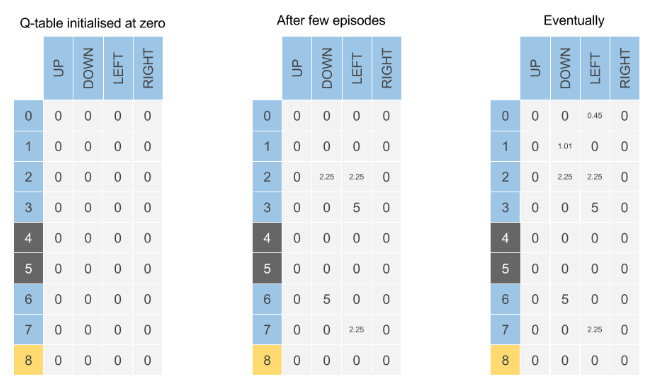
\includegraphics[height=8cm]{q_table}
	\caption{The Q-table on the left shows the initialised policy when the agent begins learning. The middle and rightmost Q-tables show the agent developing an understanding of which actions are valuable in which states.(REFERENCE)}
\end{figure}

\subsection{Deep reinforcement learning}
For low dimensional state-action spaces RL approaches result in reasonable control performance, however, as state space dimensionality increases models like Q-tables experience difficulty. The main reason for this is simply that it becomes difficult for the discrete RL algorithm to visit every state action pair resulting in unchanged values for an increasing number of state-action pairs. Essentially this means that the agent does not have complete knowledge of optimal actions for every given state, leading to the derivation of sub-optimal policies. To get around this problem, for RL problems with high dimensional state spaces, the discrete Q-table is replaced with a function approximator known as a neural network. A high level overview of the architecture can be seen in Figure 11. It is the neural network architecture in which the agent policy is implemented. As the agent learns, it adjusts weights in the neural network to change the policy. This is approach is powerful because neural networks are good at generalising, and hence the agent does not need to visit every state action pair to be able to make good decisions.
\begin{figure}[ht]
\centering
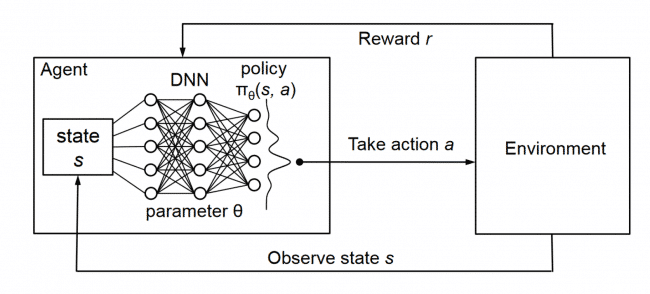
\includegraphics[height=5cm]{deep_reinforcement_learning}
\caption{The agent interacts with the environment by taking actions, which affect the state it is in and the reward it receives. The rewards allow agent to adjust the weights in the neural net to build better policies.}
\end{figure}